\section{Recovery-Aware Physical Attribution}
\label{sec:narrative-method}

Figure~\ref{fig:joint-architecture} describes the implemented computation.
The inference engine, archived as R11, uses a conditional history bank of
DAE-derived switched state-space predictors. The nonlinear simulator
generates observations; inference does not solve a new full nonlinear
simulation for every candidate at every report.

Physics enters the candidate dynamics, input directions and oriented
measurement map. Statistical filtering represents uncertain states and
discrepancy around those predictions. Thus the evaluated method is
model-based inference; it does not train a neural network with a physics
loss or learn a source-label classifier. A good residual fit alone is
insufficient: competing histories must also yield a timely source decision.

\subsection{Construct the Predictor From the Network}

Kirchhoff constraints and complex power connect sources to remote PMUs:
\begin{equation}
 I_{\rm bus}=Y_{\rm bus}V,\quad
 I_{{\rm term},r}=Y_{{\rm term},r}V,\quad S_i=V_i I_{{\rm bus},i}^{*}.
 \label{eq:narrative-electrical}
\end{equation}
Terminal rows retain orientation, line charging and transformer ratios.
A measured terminal current is not a nodal injection. A line opening
changes its branch primitive and terminal map; a load changes its admitted
P/Q input direction.

On a regular index-one DAE chart with a fixed angle reference,
\begin{align}
 \delta z&=-g_z^{-1}(g_x\delta x+g_u\delta u),\nonumber\\
 \delta\dot x&=A_q^{\rm red}\delta x+B_q^{\rm red}\delta u,\nonumber\\
 A_q^{\rm red}&=f_x-f_zg_z^{-1}g_x,\quad
 B_q^{\rm red}=f_u-f_zg_z^{-1}g_u.
 \label{eq:narrative-reduction}
\end{align}
For the instantaneous electrical observation map $H_q(x,z,u)$, the
corresponding output operators are
\begin{equation}
 C_q^{\rm red}=H_x-H_zg_z^{-1}g_x,\qquad
 D_q^{\rm red}=H_u-H_zg_z^{-1}g_u.
 \label{eq:electrical-output-reduction}
\end{equation}
They propagate a perturbation at an unmeasured source to the selected
voltage and oriented-current channels. Network connectivity enters through
the branch stamps in $g_q$ and $H_q$; eliminating unmeasured algebraic
variables generally produces dense reduced operators. The graph therefore
constrains the prediction without a learned graph embedding. A changed
terminal operator also contributes directly through $H_q$, not only
through the changed voltage. The implementation discretizes the admitted
switch modes and adds causal phase-history operators for frequency and
ROCOF. Inertia, controls and load law remain those of the fixed plant.

After augmenting instrumental memory, a conditional predictor has the
local form
\begin{align}
 \xi_{k+1}&=A_{\ell,q}\xi_k+b_{\ell,q}+B_{\ell,q}a+w_k,\nonumber\\
 r_k&=C_{\ell,q}\xi_k+d_{\ell,q}+D_{\ell,q}a+v_k.
 \label{eq:implemented-predictor}
\end{align}
Here $r_k$ contains reference-corrected, scaled and instrument-whitened PMU coordinates, $\ell$ is a fixed
network hypothesis, and $\xi_k$ contains physical deviation states, phase
history and predicted measurement-filter memory. Observed colored-instrument
filters whiten measurements; their corresponding predictor memory is
deterministic. Additional latent AR states represent persistent discrepancy,
with preset quiet/load/line/recovery covariance and drift regimes. This
statistical discrepancy model is distinct from the plant equations.
$v_k$ denotes the remaining innovation. A load has scalar severity within
its specified P/Q direction. A line uses a switched operator rather than
a fictitious load-amplitude fit. States from different equilibria are not
interpreted as an absolute rotor-state mixture.

\subsection{Estimate Context From the Startup Prefix}

Each network hypothesis uses the same 300 startup reports to estimate
operating factors, reference phase and noise scale. Voltage/current
coordinates receive a constant discrepancy correction,
\begin{equation}
 \widehat b_\ell=\overline y_{0:299}-y_\ell^{\rm ref},
 \qquad b_{\ell,k}=\widehat b_\ell\quad(k\ge300).
 \label{eq:continuous-intercept}
\end{equation}
Angular differences respect wrapping and the common reference. Frequency
and ROCOF use empirical prefix centers. The correction remains fixed so it
cannot track a later load step and subtract its signature. This estimates
an observation discrepancy, not the true impedances. Prefix estimates
enter by substitution rather than through a full joint parameter posterior.

\subsection{Compare Unknown-Onset Histories}

The method retains ten seconds of past conditional states. Its frozen
birth screen searches lags of 0--18 reports and proposes selected onsets;
it does not enumerate every onset in the 300-report history.
Each history specifies family, asset, onset,
restoration mode and severity. It starts from the stored conditional state
before its proposed onset. That state already contains any ongoing
recovery; an alarm does not reset the predictor to equilibrium.

For a retained load history, conditional Gaussian filtering yields a
residual $e$, severity response $s$ and covariance $S$. Unknown severity
has a truncated-Gaussian distribution inherited from previous reports:
\begin{equation}
 L_{h,k}=\int_l^u \mathcal N(e;sa,S)
             \operatorname{TN}_{[l,u]}(a;\mu,v)\,da.
 \label{eq:narrative-evidence}
\end{equation}
With $\Phi$ denoting the standard normal CDF, define
\begin{align}
 v'&=(v^{-1}+s^\top S^{-1}s)^{-1},\nonumber\\
 \mu'&=v'(\mu/v+s^\top S^{-1}e),\nonumber\\
 Z(\mu,v)&=\Phi((u-\mu)/\sqrt v)-\Phi((l-\mu)/\sqrt v).
\end{align}
The implemented local integral follows by completing the square:
\begin{align}
 \log L_{h,k}&=\log\mathcal N(e;0,S)+\tfrac12\log(v'/v)\nonumber\\
 &\quad+\tfrac12(\mu'^2/v'-\mu^2/v)
       +\log\frac{Z(\mu',v')}{Z(\mu,v)}.
 \label{eq:amplitude-evidence-main}
\end{align}
These standard identities are exact for the stated local conditional
model. Adaptive proposals, pruning and covariance approximations make the
complete bank approximate.

The conditional state mean is represented as $m_h+d_h a$. To make the
filtering approximation explicit, let $T_o,J_o,g_o,u_o,j_o,v_o$ denote the
archived one-report transition and observation operators for switch $o$.
The code forms $e=r_k-J_o m_h-j_o$ and $s=J_o d_h+v_o$. With the shared
covariance $P_\rho$ for the current discrepancy regime $\rho$,
\begin{align}
 S_o&=R+J_oP_\rho J_o^\top,&
 K_o&=T_oP_\rho J_o^\top S_o^{-1},\nonumber\\
 m_h^+&=T_o m_h+g_o+K_o e,&
 d_h^+&=T_o d_h+u_o-K_o s.
 \label{eq:implemented-conditional-correction}
\end{align}
The amplitude distribution is updated by the same integral above. The
regime covariances are obtained from nominal-operator Riccati equations;
R11 does not propagate an independent exact covariance for every switched
history. At episode closure, it retains the mixture mean of the augmented
state and records the omitted between-history spread. Thus state continuity
and conditional Bayesian amplitude integration are implemented, while a
fully Bayesian posterior over states, context and all histories is not.

The rolling screen proposes histories; it is not another independent
observation. Replaying a suffix replaces its original no-new-event suffix
likelihood. The sequential update therefore counts each report once,
rather than repeatedly accumulating overlapping ten-second windows.

\begin{figure*}[t]\centering
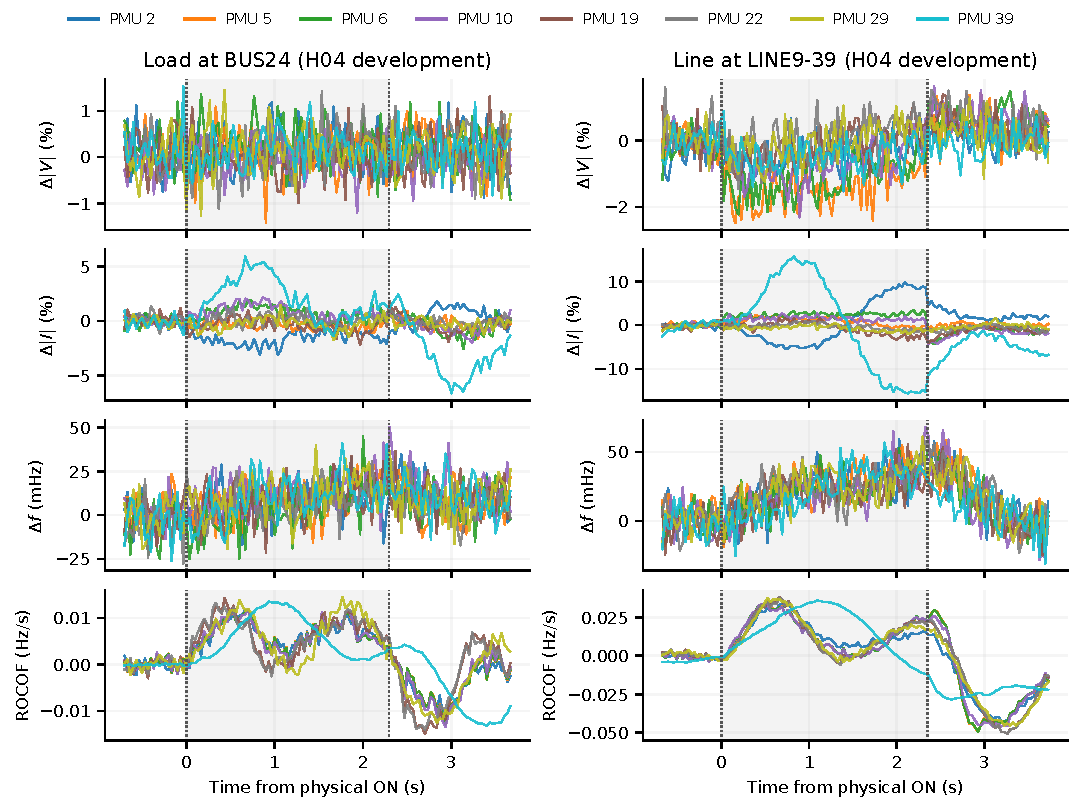
\includegraphics[width=.96\textwidth]{figures/generated/narrative_signals.pdf}
\caption{Simulated observations supplied to inference. One fixed development parent provides a load and a line example at all eight PMUs. Shading marks physical ON--OFF for evaluation only. Magnitude changes use the local pre-event center; frequency is centered for display while its exported channel remains absolute Hz. Source, severity and operating context affect the curves, so they are not universal class templates.}
\label{fig:narrative-signals}\end{figure*}

\subsection{Represent Fixed Network Uncertainty}

The bank contains nominal, global $\pm2\%$, and selected-branch $\pm3\%$
paired R/X hypotheses. Parameters stay constant within a hypothesis. Its
outer weight uses a predictive density formed before the current-report
state update and proposal selection:
\begin{equation}
 w_{\ell,k}=\frac{w_{\ell,k-1}p_\ell(y_k\mid\mathcal F_{k-1},\widehat b_\ell)}
 {\sum_jw_{j,k-1}p_j(y_k\mid\mathcal F_{k-1},\widehat b_j)}.
 \label{eq:continuous-weights}
\end{equation}
Startup-fitting reports are not scored again as independent model-selection
evidence. The mixture covers a finite set of network alternatives rather
than identifying a continuous impedance posterior.

\subsection{Keep Recovery as a Competing Physical Explanation}

Restoring an input or topology at $\kappa$ does not restore the pre-event
state: $x(\kappa^+)=x(\kappa^-)$. On a regular local post-restoration chart,
the difference from a same-context no-new-intervention trajectory obeys
\begin{align}
 \delta x_h(t)&\simeq\Phi_0(t,\kappa)\delta x_h(\kappa),\nonumber\\
 \delta y_h^{\rm net}(t)&\simeq C_0(t)\Phi_0(t,\kappa)\delta x_h(\kappa),
 \quad t>\kappa.
 \label{eq:recovery-response}
\end{align}
Here $y^{\rm net}$ denotes voltage/current coordinates before the instrument map.
Instrumental memory is retained as well. This local interpretation of known
dynamics explains why the reference after OFF is a trajectory, not a zero
residual; it is not a new propagation theorem.

For conditional history mass $\pi_{\ell,h,k}$, define active and
originating-cause masses for an admissible family/source cell $c$:
\begin{align}
 M_{c,k}&=\sum_\ell w_{\ell,k}\sum_{h:c(h)=c}
       \pi_{\ell,h,k}\,\mathbf1\{h\text{ active at }k\},\nonumber\\
 \Gamma_{c,k}&=\sum_\ell w_{\ell,k}\sum_{h:c(h)=c}\pi_{\ell,h,k}.
 \label{eq:active-cause-masses}
\end{align}
A retained history can stop being active while its cause still explains
recovery. Later interventions compete with those histories. The
implementation stores 18 admissible cells, not every family at every bus.
After confirmed episode closure, explicit histories are compressed into
the retained state mean. Cause masses describe the current bank, not a
permanent ledger of all past interventions.

Writing the conditional active mass as $M_{\ell,c,k}$ yields
\begin{align}
 \Delta M_{c,k}&=\sum_\ell w_{\ell,k}
               (M_{\ell,c,k}-M_{\ell,c,k-1})\nonumber\\
 &\quad+\sum_\ell(w_{\ell,k}-w_{\ell,k-1})M_{\ell,c,k-1}.
 \label{eq:continuous-delta}
\end{align}
The terms distinguish within-model evolution from model reweighting.
This accounting identity aids interpretation, without constituting a new
tensor factorization. The masses are approximate attribution weights;
probability calibration and globally optimal filtering are not established.

\subsection{Emit Separate Detection, Diagnosis and Restoration Messages}

The fixed publication rules require active mass 0.99 for six reports to
confirm an alarm, and restoration mass 0.99 for 15 reports to confirm OFF.
The archived source/line confirmation and episode-replacement rules
determine the public diagnosis. Every message records emission time and
the last report used. A diagnosis can be correct eventually but too late
to precede physical OFF.

The nominal comparator uses the same nominal conditional model with its
own fixed publication path. Comparing nominal and mixture evaluates two
complete configured procedures; it does not isolate the outer network bank
from publication decisions. The admission-rule ablation tests a different publication
decision; it is not a pure recovery-memory ablation.

The per-report birth and restoration hazards are
$1-\exp[-(1/60)/30]$ and $1-\exp[-(1/30)/30]$.
Birth mass is split equally between load and line families, then uniformly
among sources within each family. Load severity has a zero-mean Gaussian
prior with standard deviation 0.15, truncated to $[-0.2,0.2]$ and integrated
over four intervals with boundaries $-0.2,-0.1,0,0.1,0.2$.
After three reports, eligible active histories can produce OFF children
at either half-report position while inheriting state and severity.
After likelihood normalization, the beam retains the 96 highest-weight
recent histories, 64 older histories and at least one per occupied source;
their union is renormalized and discarded mass is recorded.
The reproducibility archive maps these operations to the frozen
\texttt{transitions}, \texttt{process}, and
\texttt{predictive\_log\_density} routines and preserves the complete
publication configuration.

\subsection{Per-Report Algorithm and Computational Boundary}

\noindent\textbf{Algorithm 1: causal physical-history attribution.}
The inputs are the nominal model, fixed method configuration and successive
PMU reports. Reserved event truth never enters these steps.
\begin{enumerate}
\item Estimate operating context, common reference and noise scale from the
startup prefix. Initialize conditional states and retain the eligible past
states needed by retrospective proposals.
\item At report $k$, apply the frozen centering, scaling and instrumental
transformation. Propagate each retained physical/recovery history and its
conditional uncertainty to predict this report. Compute and save the outer
model predictive density before current-report screening and state correction.
\item Apply the frozen short-lag birth screen using retained past states.
A proposed history starts before its selected onset; replay
replaces the corresponding likelihood suffix rather than adding it twice.
\item Score candidate histories and replayed suffixes before correcting
their states with the reports being scored. Integrate the allowed load severity and apply
the archived switched operator for a line hypothesis.
\item Correct the conditional states and severity distributions; update
network weights and the retained history bank using the fixed rules.
Preserve dynamic state and originating cause through restoration.
\item Aggregate active mass $M$, cause mass $\Gamma$ and $\Delta M$.
Apply the fixed alarm, diagnosis and OFF-publication rules. Store emission
time, estimated onset, family/source and the last report used.
\end{enumerate}
The nonlinear simulator constructs observations; this algorithm propagates
local switched predictors. The input grid is 30 reports/s. Causality
concerns report availability; acquisition throughput, computation time
and the electrical history needed for a decision are separate quantities.
Wall-clock real-time operation has not been established.
